\section{Results}
\label{sec:results}

All numbers below are read from the committed result files; the figure and table scripts in \file{report/ieee/} regenerate every artefact from those files. Values are reported to the precision of the source.

\subsection{Tokenizer-level diagnostics}
\label{sec:res:tokenizer}
Fig.~\ref{fig:tokenizer} and Table~\ref{tab:tokenizer} characterise the three tokenizers on 5{,}000 Azerbaijani Wikipedia sentences (102{,}726 words) and on the 27{,}914 task examples. \xlmxv{} segments Azerbaijani into 3.21 tokens per word, \xlmr{} into 1.90, and the donor into 1.76; the \xlmxv{} deficit is structural, because its lower-cased, accent-stripped fastBPE vocabulary contains no token bearing ş, ç, ö, ü or ğ and only two containing ə, whereas \xlmr{} and the donor contain thousands (pre-grid vocabulary counts, \file{diacritics.json}). At the frozen maximum length of 256 tokens, 1.257\% of task examples are truncated under \xlmxv{}, 0.473\% under \xlmr{}, and 0.351\% under the donor; the transplant therefore also changes how much text the encoder sees, a confound of at most 0.9 percentage points of examples.

Alphabetic token-type overlap between Azerbaijani and four other languages (Fig.~\ref{fig:tokenizer}b) shows that Turkish covers more Azerbaijani types than English or Finnish for every vocabulary---66.7\% vs.\ a 58.2\% Latin-script baseline for \xlmxv{} (+8.5~pt), 46.4\% vs.\ 33.8\% for \xlmr{} (+12.6~pt), 32.1\% vs.\ 19.2\% for the donor (+12.9~pt)---while Cyrillic-script Russian covers 8–17\%. The English–Finnish spread is at most 1.6~pt, so the Turkish lift is not noise, but the Russian comparison shows that script alone moves overlap by tens of points; overlap is a lexical-similarity signal, not evidence of linguistic transfer, and it is the reason a lexical-only explanation of any Turkish benefit cannot be excluded by design.

\begin{figure*}[!t]
\centering
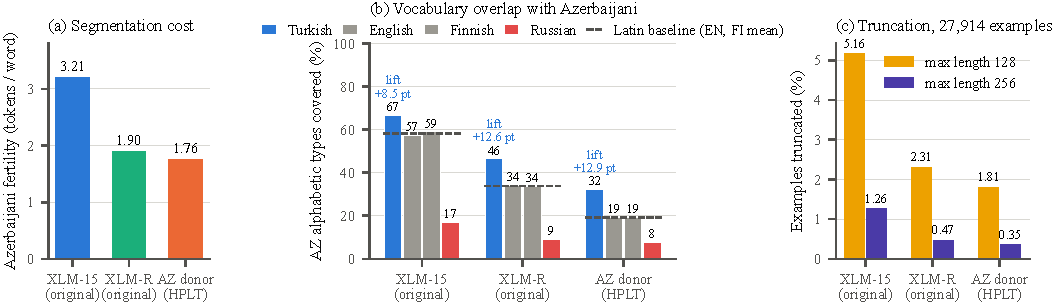
\includegraphics[width=\textwidth]{figures/fig_tokenizer.pdf}
\caption{Tokenizer diagnostics. (a) Azerbaijani fertility on 5{,}000 Wikipedia sentences (\file{results/overlap\_control.json}). (b) Share of Azerbaijani alphabetic token types also present in the tokenization of 5{,}000 sentences of Turkish, English, Finnish and Russian; the dashed line is the English–Finnish mean, the annotated lift is Turkish minus that baseline. (c) Share of the 27{,}914 task examples truncated at maximum length 128 and 256 (\file{results/truncation.json}); 256 is the frozen setting.}
\label{fig:tokenizer}
\end{figure*}

\begin{table*}[!t]
\caption{Tokenizer diagnostics. Fertility, alphabetic types and overlap from \file{results/overlap\_control.json} (5{,}000 Wikipedia sentences per language); letter counts are the number of vocabulary entries containing the letter (\file{evidence/carried\_forward\_pre\_grid/diacritics.json}, pre-grid, dataset-level); token-length statistics and truncation from \file{results/truncation.json} on the 27{,}914 task examples. Lift = Turkish overlap minus the English–Finnish mean.}
\label{tab:tokenizer}
\centering
\footnotesize
\begin{tabular}{@{}lrrrrrrrrrrrrrrr@{}}
\toprule
 & & & AZ alpha. & \multicolumn{4}{c}{AZ types covered by (\%)} & & \multicolumn{3}{c}{Vocab.\ entries with} & \multicolumn{2}{c}{Task tokens} & \multicolumn{2}{c}{Truncated (\%)} \\
\cmidrule(lr){5-8}\cmidrule(lr){10-12}\cmidrule(lr){13-14}\cmidrule(lr){15-16}
Tokenizer & Vocab & Fertility & types & TR & EN & FI & RU & Lift & ə & ş & ğ & mean & p99 & 128 & 256 \\
\midrule
% AUTO-GENERATED by report/ieee/tables/make_tables.py -- do not edit by hand.
% source: results/overlap_control.json
% source: results/truncation.json
% source: evidence/carried_forward_pre_grid/diacritics.json (pre-grid vocabulary letter counts)
XLM-15 & 95,000 & 3.206 & 3,257 & 66.7 & 57.4 & 59.0 & 16.8 & +8.5 & 2 & 0 & 0 & 49.0 & 283 & 5.16 & 1.26 \\
XLM-R & 250,002 & 1.904 & 10,054 & 46.4 & 34.1 & 33.6 & 9.0 & +12.6 & 1,366 & 891 & 407 & 33.7 & 189 & 2.31 & 0.47 \\
AZ donor & 32,770 & 1.758 & 14,858 & 32.1 & 19.3 & 19.1 & 7.7 & +12.9 & 8,814 & 2,253 & 928 & 30.3 & 169 & 1.81 & 0.35 \\
\bottomrule

\end{tabular}
\end{table*}

\subsection{Intrinsic transplant diagnostics}
\label{sec:res:intrinsic}
Before any downstream training, each transplanted artefact was probed on a deterministic 300-line sample of Azerbaijani \emph{training} text (validation and test untouched) with three intrinsic measures (Table~\ref{tab:intrinsic}, Fig.~\ref{fig:intrinsic}): masked-token top-1 accuracy of the masked-LM head, bits per character (BPC), and the embedding-norm ratio before rescaling. BPC rather than perplexity is used because different tokenizers split the same text into different numbers of tokens; BPC normalises the masked-LM loss by characters:
\begin{equation}
\mathrm{BPC}=\frac{\ell_{\mathrm{MLM}}\cdot N_{\mathrm{tok}}}{N_{\mathrm{char}}\ln 2},
\label{eq:bpc}
\end{equation}
with $\ell_{\mathrm{MLM}}$ the mean loss per masked token in nats.

The two bases behave very differently. \xlmr{}'s original masked-LM head predicts 602 of 1{,}631 masked Azerbaijani tokens (36.91\%) at 1.60 BPC; after OMP transplantation it predicts 40 of 1{,}502 (2.66\%) at 6.94 BPC ($\Delta=+5.34$), and the raw reconstruction inflated row norms by $1.91\times$ before rescaling, outside the healthy band of $[0.85, 1.15]$ defined in the norm report. The placebos are worse still ($\Delta$BPC $+5.53$ for \Mean{}, $+7.06$ for \Random{}), so OMP is the \emph{best} of the three initialisers on \xlmr{} while remaining far from the original. \xlmxv{}'s original head is already near chance on Azerbaijani (2 of 2{,}323, 0.09\%; 7.21 BPC), and its OMP transplant stays at 2 of 1{,}502 with a \emph{lower} BPC of 6.00 ($\Delta=-1.20$) and a healthy norm ratio of 1.13. As the quality file itself warns, a BPC decrease at near-zero top-1 accuracy is a calibration change over a smaller vocabulary, not recovered lexical knowledge; the two measures must be read together. Eligible masked positions differ between tokenizers, so these are diagnostics rather than paired token-level accuracies. The independent signals---top-1 collapse, BPC increase, and norm inflation---all point to the same conclusion the downstream grid reaches for \xlmr{}: the implemented reconstruction does not preserve the information the encoder expects in its embedding rows.

\begin{table*}[!t]
\caption{Intrinsic diagnostics of the installed artefacts on 300 Azerbaijani training lines (\file{results/controls\_\_\{base\}\_\_\{tag\}.json}). Top-1 is correct/masked positions; BPC per Eq.~\eqref{eq:bpc}; the norm ratio is reconstructed-to-anchor median norm of the raw OMP reconstruction \emph{before} Eq.~\eqref{eq:rescale} (\file{embedding\_norm\_report}); all installed artefacts are rescaled to 1.000.}
\label{tab:intrinsic}
\centering
\footnotesize
\begin{tabular}{@{}llrrrrrr@{}}
\toprule
 & & \multicolumn{2}{c}{Top-1 (correct/masked)} & \multicolumn{3}{c}{BPC} & Pre-rescale \\
\cmidrule(lr){3-4}\cmidrule(lr){5-7}
Base & Init. & original & transplanted & original & transpl. & $\Delta$ & norm ratio \\
\midrule
% AUTO-GENERATED by report/ieee/tables/make_tables.py -- do not edit by hand.
% source: results/controls__{base}__{tag}.json (C1c)
% source: results/embedding_norm_report__{base}.json (pre-rescale norm ratio)
XLM-15 & OMP & 2/2,323 & 2/1,502 & 7.2071 & 6.0034 & -1.2037 & 1.1324 \\
XLM-15 & Mean & 2/2,323 & 0/1,502 & 7.2071 & 6.0763 & -1.1308 & -- \\
XLM-15 & Random & 2/2,323 & 6/1,502 & 7.2071 & 8.1814 & +0.9743 & -- \\
\midrule
XLM-R & OMP & 602/1,631 & 40/1,502 & 1.5975 & 6.9352 & +5.3377 & 1.9091 \\
XLM-R & Mean & 602/1,631 & 19/1,502 & 1.5975 & 7.1276 & +5.5301 & -- \\
XLM-R & Random & 602/1,631 & 16/1,502 & 1.5975 & 8.6611 & +7.0636 & -- \\
\bottomrule

\end{tabular}
\end{table*}

\begin{figure*}[!t]
\centering
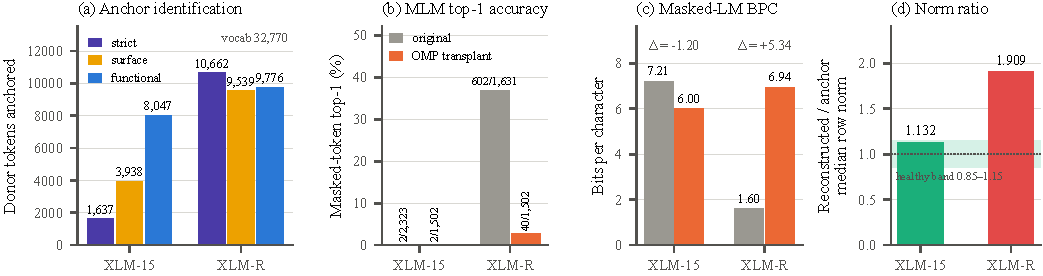
\includegraphics[width=\textwidth]{figures/fig_intrinsic.pdf}
\caption{Intrinsic transplant diagnostics. (a) Anchors found by the three identification modes (\file{results/anchors.json}); functional mode is the pre-registered default. (b) Masked-token top-1 accuracy of the original and the OMP-transplanted masked-LM head on the same 300 training lines (\file{results/top1\_accuracy.json}). (c) Bits per character (\file{results/cross\_base\_transplant\_quality.json}). (d) Reconstructed-to-anchor median-norm ratio of the raw OMP reconstruction with the healthy band of the norm report (\file{results/embedding\_norm\_report\_\_*.json}); the installed artefacts were rescaled to 1.000.}
\label{fig:intrinsic}
\end{figure*}

\subsection{Reference-size grid}
\label{sec:res:grid}
Tables~\ref{tab:results2000} and~\ref{tab:results500} report every cell at the two primary sizes on validation and on test; Appendix~\ref{app:cells} adds the confidence intervals and the higher-data cells. Two facts organise everything that follows. First, \xlmr{} escapes in every one of its 70 runs, so its conditional and all-seed estimands coincide and every \xlmr{} contrast is measurable. Second, \xlmxv{} escapes in 60 of 94 runs, between 2/5 and 5/5 per cell at the primary sizes, so its two estimands diverge by up to 0.21 and its conditional means describe different survivor subsets in different conditions.

For \xlmr{} at $n=2{,}000$, \OMP{} minus \Direct{} is $-0.0659$ on validation (0.8277$\to$0.7618) and $-0.0566$ on test (0.7970$\to$0.7404); at $n=500$ the effects are $-0.0782$ and $-0.0748$. \Mean{} ($-0.0505$, $-0.0560$) and \Random{} ($-0.0980$, $-0.0996$) also underperform \Direct{} at both sizes, with \Random{} worst, and \OMP{} sits between them: better than \Random{} by $+0.032$ and $+0.021$, worse than \Mean{} by $-0.016$ and $-0.022$. \TR{} is the numerically best \xlmr{} condition at both sizes (0.8307 and 0.8149 on validation; 0.8048 and 0.7910 on test), followed by \ShufTR{} and \Direct{}; \OMPTR{} lies between \OMP{} and \Mean{}. For \xlmxv{}, conditional means at $n=2{,}000$ lie within 0.61–0.70 for every condition while all-seed means range from 0.48 (\Direct, 2/5 escaped) to 0.67 (\OMPTR, 5/5); the ordering of conditions depends on which estimand is chosen.

\begin{table*}[!t]
\caption{Complete results at $n=2{,}000$. Escape is escaped/declared seeds; conditional \Fone{} averages escaped seeds only (10{,}000-resample percentile bootstrap 95\% CI); all-seed \Fone{} charges collapsed seeds at their actual score; test values are from the restored validation-selected checkpoint; TR deg.\ counts degenerate Turkish source stages (\file{results/summary.csv}, T1 of \file{evidence/supplemental/test\_tables\_received.md}).}
\label{tab:results2000}
\centering
\footnotesize
\begin{tabular}{@{}llcrlrrrc@{}}
\toprule
 & & & \multicolumn{3}{c}{Validation \Fone} & \multicolumn{2}{c}{Test \Fone} & \\
\cmidrule(lr){4-6}\cmidrule(lr){7-8}
Base & Condition & Escape & cond. & 95\% CI & all-seed & cond. & all-seed & TR deg. \\
\midrule
% AUTO-GENERATED by report/ieee/tables/make_tables.py -- do not edit by hand.
% source: results/summary.csv
% source: evidence/supplemental/test_tables_received.md (T1)
% source: results/runs/*.json
XLM-15 & Direct & 2/5 & 0.6791 & [0.674, 0.684] & 0.4799 & 0.6735 & 0.4790 & 0 \\
XLM-15 & OMP & 3/5 & 0.6148 & [0.464, 0.691] & 0.5023 & 0.6076 & 0.4980 & 0 \\
XLM-15 & Mean & 3/5 & 0.6955 & [0.675, 0.706] & 0.5507 & 0.6833 & 0.5434 & 0 \\
XLM-15 & Random & 4/5 & 0.6699 & [0.664, 0.673] & 0.6026 & 0.6529 & 0.5890 & 0 \\
XLM-15 & TR & 4/5 & 0.6747 & [0.661, 0.687] & 0.6064 & 0.6663 & 0.5997 & 2 \\
XLM-15 & OMP+TR & 5/5 & 0.6712 & [0.645, 0.689] & 0.6712 & 0.6645 & 0.6645 & 3 \\
XLM-15 & Shuf. TR & 2/5 & 0.6873 & [0.682, 0.692] & 0.4750 & 0.6784 & 0.4714 & 2 \\
\midrule
XLM-R & Direct & 5/5 & 0.8277 & [0.823, 0.833] & 0.8277 & 0.7970 & 0.7970 & 0 \\
XLM-R & OMP & 5/5 & 0.7618 & [0.755, 0.769] & 0.7618 & 0.7404 & 0.7404 & 0 \\
XLM-R & Mean & 5/5 & 0.7772 & [0.772, 0.783] & 0.7772 & 0.7578 & 0.7578 & 0 \\
XLM-R & Random & 5/5 & 0.7297 & [0.725, 0.735] & 0.7297 & 0.7154 & 0.7154 & 0 \\
XLM-R & TR & 5/5 & 0.8307 & [0.829, 0.832] & 0.8307 & 0.8048 & 0.8048 & 0 \\
XLM-R & OMP+TR & 5/5 & 0.7708 & [0.766, 0.776] & 0.7708 & 0.7546 & 0.7546 & 0 \\
XLM-R & Shuf. TR & 5/5 & 0.8269 & [0.825, 0.829] & 0.8269 & 0.7971 & 0.7971 & 0 \\
\bottomrule

\end{tabular}
\end{table*}

\begin{table*}[!t]
\caption{Complete results at $n=500$; columns as in Table~\ref{tab:results2000}.}
\label{tab:results500}
\centering
\footnotesize
\begin{tabular}{@{}llcrlrrrc@{}}
\toprule
 & & & \multicolumn{3}{c}{Validation \Fone} & \multicolumn{2}{c}{Test \Fone} & \\
\cmidrule(lr){4-6}\cmidrule(lr){7-8}
Base & Condition & Escape & cond. & 95\% CI & all-seed & cond. & all-seed & TR deg. \\
\midrule
% AUTO-GENERATED by report/ieee/tables/make_tables.py -- do not edit by hand.
% source: results/summary.csv
% source: evidence/supplemental/test_tables_received.md (T1)
% source: results/runs/*.json
XLM-15 & Direct & 3/5 & 0.6306 & [0.621, 0.639] & 0.5117 & 0.6229 & 0.5071 & 0 \\
XLM-15 & OMP & 2/5 & 0.5272 & [0.440, 0.614] & 0.4109 & 0.5248 & 0.4100 & 0 \\
XLM-15 & Mean & 2/5 & 0.6359 & [0.627, 0.645] & 0.4544 & 0.6302 & 0.4521 & 0 \\
XLM-15 & Random & 3/5 & 0.6192 & [0.609, 0.632] & 0.5049 & 0.6025 & 0.4949 & 0 \\
XLM-15 & TR & 4/5 & 0.6141 & [0.575, 0.639] & 0.5580 & 0.6090 & 0.5539 & 2 \\
XLM-15 & OMP+TR & 5/5 & 0.6217 & [0.611, 0.630] & 0.6217 & 0.6142 & 0.6142 & 3 \\
XLM-15 & Shuf. TR & 3/5 & 0.6348 & [0.620, 0.646] & 0.5143 & 0.6336 & 0.5135 & 2 \\
\midrule
XLM-R & Direct & 5/5 & 0.7980 & [0.794, 0.804] & 0.7980 & 0.7783 & 0.7783 & 0 \\
XLM-R & OMP & 5/5 & 0.7198 & [0.710, 0.728] & 0.7198 & 0.7035 & 0.7035 & 0 \\
XLM-R & Mean & 5/5 & 0.7421 & [0.732, 0.752] & 0.7421 & 0.7217 & 0.7217 & 0 \\
XLM-R & Random & 5/5 & 0.6985 & [0.688, 0.709] & 0.6985 & 0.6867 & 0.6867 & 0 \\
XLM-R & TR & 5/5 & 0.8149 & [0.810, 0.819] & 0.8149 & 0.7910 & 0.7910 & 0 \\
XLM-R & OMP+TR & 5/5 & 0.7261 & [0.708, 0.741] & 0.7261 & 0.7173 & 0.7173 & 0 \\
XLM-R & Shuf. TR & 5/5 & 0.8054 & [0.799, 0.810] & 0.8054 & 0.7814 & 0.7814 & 0 \\
\bottomrule

\end{tabular}
\end{table*}

\subsection{Optimisation failure: escape, collapse, and dynamics}
\label{sec:res:escape}
Fig.~\ref{fig:trajectories} shows the ten validation points of all 70 runs at $n=2{,}000$. Every \xlmr{} run leaves the collapse basin by the first or second evaluation (68 of 70 at step 200, 2 at step 400) and then changes little, which is why its seeds cluster tightly. \xlmxv{} behaves qualitatively differently: 34 of its 94 runs never leave the basin, escapes are spread from step 200 to step 2{,}000 with a mode at 400 (Fig.~\ref{fig:escape}a), and individual runs can leave the basin, fall back into it, and leave again (\TR, seed 42: 0.42 at step 600, $1/3$ at steps 800–1{,}600, 0.65 at step 2{,}000). Two runs crossed the threshold mid-training and ended collapsed (\OMP{} and \Mean{} at $n=500$); they are legitimately ``escaped'' under Eq.~\eqref{eq:escape} while their selected checkpoint is an early one, and the schema records them as such (\pfx{escaped\_but\_terminal\_collapsed}). Collapse is a one-class output: 32 of the 34 collapsed runs predict the negative class for every one of the 4{,}186 test examples and the remaining two predict it for almost all (Fig.~\ref{fig:escape}b), giving test \Fone{} of 0.333–0.387.

No escape-rate difference between conditions is significant: across all 96 declared contrasts the smallest Fisher exact $p$ is 0.167 (\Direct{} 2/5 vs.\ \OMPTR{} 5/5 on \xlmxv{} at $n=2{,}000$). With five seeds per cell, escape probabilities cannot be resolved beyond the Wilson intervals shown in Fig.~\ref{fig:summary}a; this is a design limit stated in advance, not a post hoc finding.

\begin{figure*}[!t]
\centering
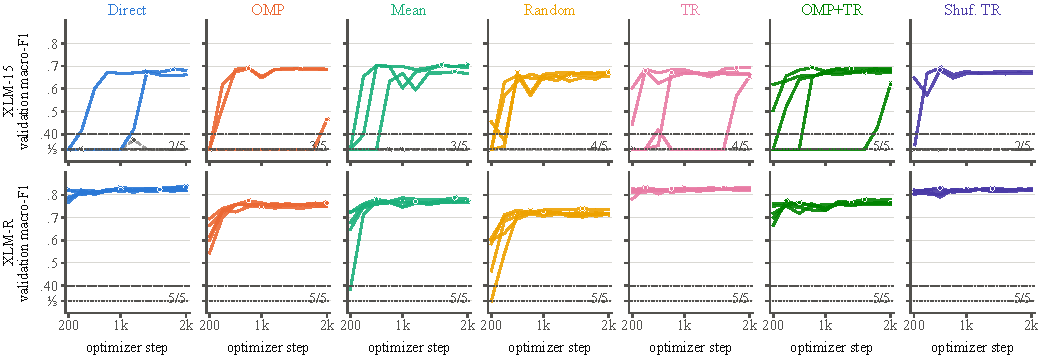
\includegraphics[width=\textwidth]{figures/fig_trajectories.pdf}
\caption{Validation \Fone{} at the ten evaluation points (steps 200–2{,}000) of all 70 runs at $n=2{,}000$, one panel per base and condition, one line per seed (\file{results/runs/*\_\_n=2000\_\_*.json}, \pfx{step\_history}). Coloured solid lines escaped; grey dashed lines never crossed the threshold. The dot marks the selected checkpoint $t^\ast$; the dotted line is the collapse basin ($1/3$), the dash-dotted line the escape threshold (0.40); the corner number is escaped/declared seeds.}
\label{fig:trajectories}
\end{figure*}

\begin{figure}[!t]
\centering
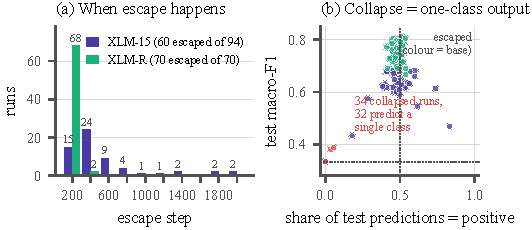
\includegraphics[width=\columnwidth]{figures/fig_escape.pdf}
\caption{Escape and collapse over all 164 runs (\file{results/runs/*.json}). (a) Step at which validation \Fone{} first exceeded 0.40 for the 130 escaped runs. (b) Share of positive predictions on the test split against test \Fone; collapsed runs (red) sit at a single-class output with \Fone{}$\approx1/3$.}
\label{fig:escape}
\end{figure}

\begin{figure*}[!t]
\centering
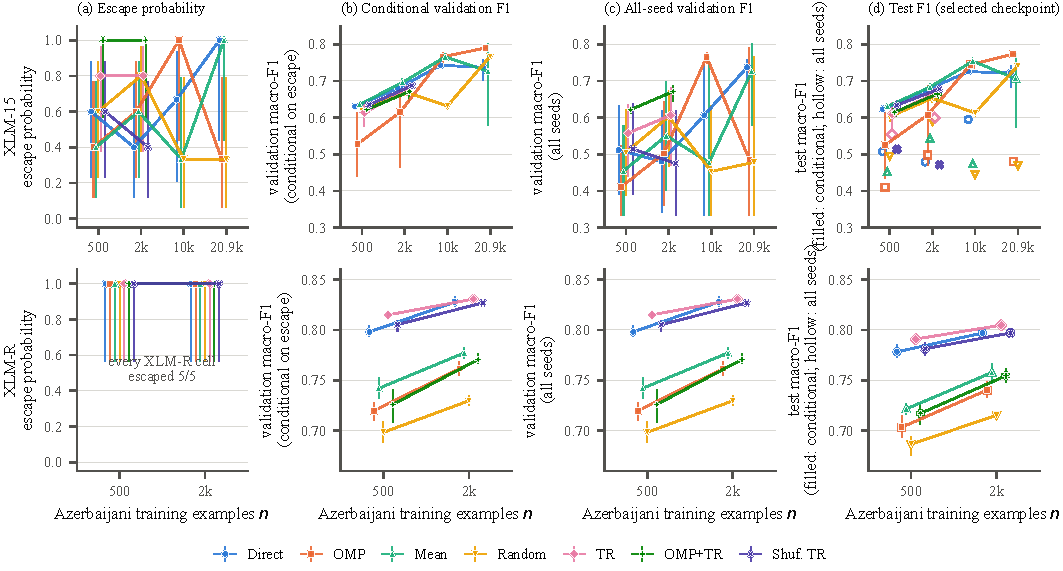
\includegraphics[width=\textwidth]{figures/fig_summary.pdf}
\caption{Failure-aware summary across Azerbaijani training sizes (top: \xlmxv; bottom: \xlmr). (a) Escape probability with Wilson 95\% intervals; every \xlmr{} cell escaped 5/5. (b) Validation \Fone{} conditional on escape and (c) over all seeds, with 10{,}000-resample percentile-bootstrap intervals (\file{results/summary.csv}). (d) Test \Fone{} at the validation-selected checkpoint, conditional (filled, with CI) and all-seed (hollow) (T1 of \file{test\_tables\_received.md}). Lines connect matched conditions and are visual guides; the size axis is a fixed-budget stress test, not a learning curve.}
\label{fig:summary}
\end{figure*}

\subsection{Direct-relative effects and multiplicity control}
\label{sec:res:effects}
Table~\ref{tab:contrastsxlmr} and Fig.~\ref{fig:forest} report every within-base contrast for \xlmr{}, where all seeds escaped and the conditional Welch family is fully measurable. Of the 86 measurable contrasts in the pre-registered family (all 42 \xlmr{} contrasts and 44 of the 54 \xlmxv{} contrasts), 27 survive Holm correction; every survivor is an \xlmr{} contrast (12 at $n=500$, 15 at $n=2{,}000$), and none involves \xlmxv, whose smallest raw Welch $p$ is 0.107. The survivors are the contrasts that separate the four donor-tokenizer arms (\OMP, \Mean, \Random, \OMPTR) from the three original-tokenizer arms (\Direct, \TR, \ShufTR)---all twelve such pairs at $n=2{,}000$ and eleven of twelve at $n=500$, where \Direct$	o$\OMPTR{} misses at Holm $p=0.063$---plus the within-transplant orderings that place \Random{} below \Mean{} at both sizes and below \OMP{} and \OMPTR{} at $n=2{,}000$. \OMP{} versus \Mean{} does not survive at either size. Every one of the six Direct-relative transplant contrasts (three initialisers at two sizes) survives, with Cohen's $d$ between $-5.3$ and $-14.9$ and bootstrap intervals excluding zero; the Holm-adjusted $p$ for \Direct$\to$\OMP{} is $7.6\times10^{-4}$ at $n=500$ and below $10^{-5}$ at $n=2{,}000$.

Turkish intermediate training is not a resolved Direct-relative improvement. \TR{} minus \Direct{} on \xlmr{} is $+0.0169$ at $n=500$ (Welch $p=0.0034$, Holm-adjusted $p=0.1955$; paired diagnostic $p=0.0021$) and $+0.0030$ at $n=2{,}000$ (Welch $p=0.372$); the corresponding test differences are $+0.0127$ and $+0.0078$. The $n=500$ direction is 5.6 times the $n=2{,}000$ direction, which is compatible with the low-resource pattern reported by Kardeş-NLU, but the current seed count does not resolve it after correction for the family it belongs to. Real versus shuffled Turkish differs by $+0.0096$ at $n=500$ (Welch $p=0.048$, Holm 1) and $+0.0038$ at $n=2{,}000$ (Welch $p=0.038$, Holm 1): the order-sensitive component (H1) is directionally positive and small, and not established. \ShufTR{} is itself indistinguishable from \Direct{} ($+0.0073$ and $-0.0008$). The interaction contrasts are informative in one direction only: \OMPTR{} is below \TR{} by $-0.0889$ and $-0.0599$ (both survive), showing that the transplant offsets the stronger original-tokenizer outcome; \OMPTR{} versus \OMP{} ($+0.0062$, $+0.0090$; Holm 1) does not show that Turkish knowledge failed or succeeded in transferring through donor rows.

\begin{table*}[!t]
\caption{Direct-relative contrasts on \xlmr{} (\file{results/stats.csv}). $\Delta$ is conditional validation \Fone{} (comparison minus \Direct) with its bootstrap 95\% CI; Welch $p$ is raw, Holm $p$ is adjusted over the 86-test family; paired $p$ is the same-seed diagnostic; $\Delta$ test is the paired test difference (T2 of \file{test\_tables\_received.md}); \checkmark{} marks family survivors.}
\label{tab:contrastsxlmr}
\centering
\footnotesize
\begin{tabular}{@{}rlrlrrrrrc@{}}
\toprule
$n$ & Contrast & $\Delta$ val & 95\% CI & Welch $p$ & Holm $p$ & Paired $p$ & $d$ & $\Delta$ test & Surv. \\
\midrule
% AUTO-GENERATED by report/ieee/tables/make_tables.py -- do not edit by hand.
% source: results/stats.csv
% source: test_tables_received.md (T2)
500 & Direct $\to$ OMP & -0.0782 & [-0.090, -0.068] & 1.0e-5 & 7.6e-4 & 3.5e-4 & -7.99 & -0.0748 & \checkmark \\
500 & Direct $\to$ Mean & -0.0560 & [-0.068, -0.044] & 1.4e-4 & 0.0090 & 0.0026 & -5.31 & -0.0566 & \checkmark \\
500 & Direct $\to$ Random & -0.0996 & [-0.112, -0.088] & 1.0e-5 & 7.6e-4 & 2.0e-4 & -9.39 & -0.0917 & \checkmark \\
500 & Direct $\to$ TR & +0.0169 & [+0.009, +0.024] & 0.0034 & 0.1955 & 0.0021 & +2.64 & +0.0127 &  \\
500 & Direct $\to$ OMP+TR & -0.0720 & [-0.092, -0.056] & 0.0011 & 0.0631 & 0.0045 & -4.43 & -0.0610 &  \\
500 & Direct $\to$ Shuf. TR & +0.0073 & [-0.001, +0.014] & 0.1386 & 1 & 0.1091 & +1.04 & +0.0031 &  \\
\midrule
2,000 & Direct $\to$ OMP & -0.0659 & [-0.075, -0.057] & $<$1e-5 & $<$1e-5 & 4.0e-5 & -8.31 & -0.0566 & \checkmark \\
2,000 & Direct $\to$ Mean & -0.0505 & [-0.058, -0.043] & $<$1e-5 & $<$1e-5 & 3.9e-4 & -7.53 & -0.0392 & \checkmark \\
2,000 & Direct $\to$ Random & -0.0980 & [-0.105, -0.091] & $<$1e-5 & $<$1e-5 & 2.0e-5 & -14.86 & -0.0816 & \checkmark \\
2,000 & Direct $\to$ TR & +0.0030 & [-0.003, +0.008] & 0.3721 & 1 & 0.3755 & +0.62 & +0.0078 &  \\
2,000 & Direct $\to$ OMP+TR & -0.0569 & [-0.064, -0.050] & $<$1e-5 & $<$1e-5 & 2.9e-4 & -8.88 & -0.0424 & \checkmark \\
2,000 & Direct $\to$ Shuf. TR & -0.0008 & [-0.006, +0.004] & 0.8026 & 1 & 0.8254 & -0.17 & +0.0001 &  \\
\bottomrule

\end{tabular}
\end{table*}

\begin{figure*}[!t]
\centering
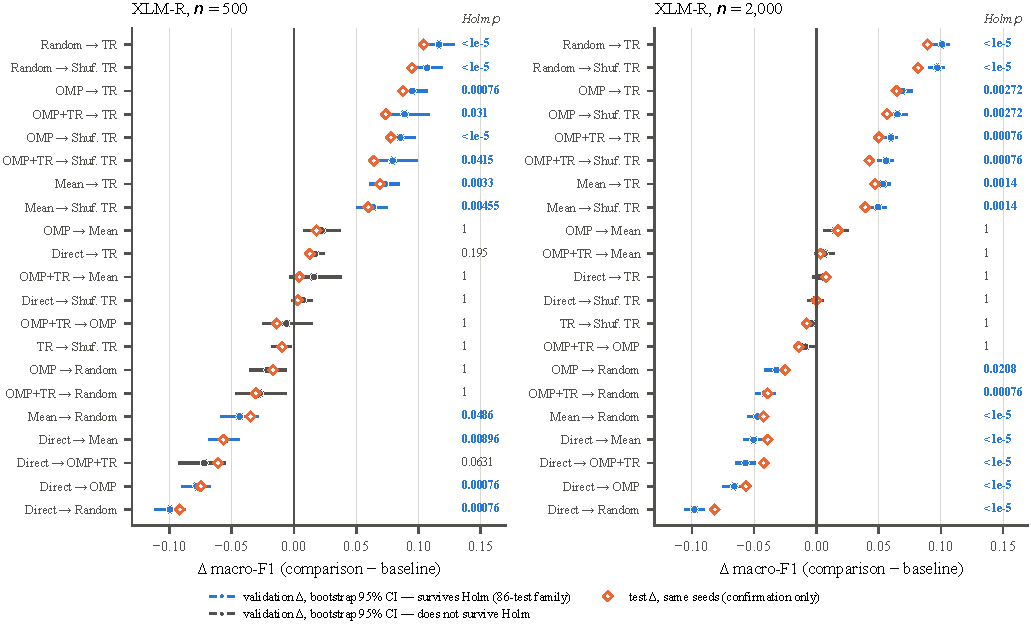
\includegraphics[width=0.95\textwidth]{figures/fig_forest.pdf}
\caption{All 42 within-base \xlmr{} contrasts (comparison minus baseline). Circles: conditional validation difference with 10{,}000-resample bootstrap 95\% CI (\file{results/stats.csv}); blue if the contrast survives Holm correction over the 86-test family, grey otherwise, with the Holm-adjusted $p$ printed at right. Hollow diamonds: paired test difference on the same five seeds (recomputed from \file{results/runs/*.json}; identical to T2/T5 of \file{test\_tables\_received.md}). Test values are confirmation only and were not used to select contrasts.}
\label{fig:forest}
\end{figure*}

\subsection{Test-side confirmation of validation-selected contrasts}
\label{sec:res:confirm}
The 27 survivors were fixed by the validation analysis and then re-tested on the held-out split with a paired $t$ over the same five seeds, Holm-corrected within the 27 (Appendix~\ref{app:survivors}). All 27 retain their sign and remain significant on test (largest within-family Holm-adjusted $p$: $1.72\times10^{-2}$, for \Mean$\to$\Random{} at $n=500$); the mean test-to-validation absolute-effect ratio is 0.874, i.e., effects shrink slightly, as expected for a checkpoint selected on validation. Across the broader set of 38 paired contrasts (both bases, any shared escaped seed), validation and test differences agree in sign for 33, and for 26 of the 27 with $|\Delta_{\mathrm{val}}|\ge0.01$; the Pearson correlation between $\Delta_{\mathrm{val}}$ and $\Delta_{\mathrm{test}}$ is 0.9898 (Fig.~\ref{fig:valtest}c). Every sign disagreement occurs where $|\Delta_{\mathrm{val}}|<0.01$ or where fewer than three seeds escaped in both arms. These calculations assess stability of the validation-selected conclusions; they do not convert the test split into a second discovery set.

\subsection{The exact sign-flip floor}
\label{sec:res:exact}
The paired $t$ statistics behind the confirmation are large (up to $|t|=61$, $p$ down to $4\times10^{-7}$) because the five seed differences are unanimous and tightly clustered. Those $p$-values rest on the normal model. Under exact sign-flip inference, Eq.~\eqref{eq:signflip}, five paired seeds admit 32 assignments and the smallest attainable two-sided $p$ is $2/32=0.0625$. All 27 survivors attain that floor on validation and on test, and all five seed differences point the same way in all 27 contrasts on both splits (Fig.~\ref{fig:signflip}): this is the maximum evidence a five-seed design can produce, and it cannot satisfy $p<0.05$ without a distributional assumption. More seeds are the only direct remedy; additional post hoc tests on the same five runs are not.

\begin{figure}[!t]
\centering
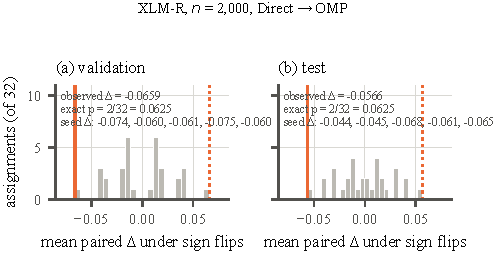
\includegraphics[width=\columnwidth]{figures/fig_signflip.pdf}
\caption{Exact sign-flip distribution for the headline contrast (\xlmr, $n=2{,}000$, \Direct$\to$\OMP), recomputed from the five per-seed differences in \file{results/runs/*.json}. The observed mean difference (solid line) and its mirror (dotted) are the two most extreme of the 32 assignments on both splits, so $p_{\mathrm{exact}}=2/32=0.0625$; the seed-level differences are printed in each panel.}
\label{fig:signflip}
\end{figure}

\subsection{Turkish source stage and degeneracy}
\label{sec:res:turkish}
Fourteen of the 30 \xlmxv{} Turkish source stages are degenerate---4 of 10 for \TR, 6 of 10 for \OMPTR, 4 of 10 for \ShufTR{} (seven at each Azerbaijani size)---with three-class Turkish \Fone{} of 0.16–0.38, i.e., the source classifier predicted one or two classes; none of the 30 \xlmr{} stages is degenerate (Turkish \Fone{} 0.69–0.79) (Fig.~\ref{fig:turkish}a). Downstream escape occurs after incompetent source stages as well as after competent ones (Fig.~\ref{fig:turkish}b), so source-stage and target-stage success are not interchangeable, and any statement that Turkish training ``stabilises'' \xlmxv{} (5/5 escapes for \OMPTR{} at both sizes) must carry the degeneracy count. Table~\ref{tab:turkish} collects the Turkish-related contrasts for both bases; on \xlmxv{} none approaches significance, and paired diagnostics are often unavailable because fewer than two seeds escaped in both arms.

\begin{figure}[!t]
\centering
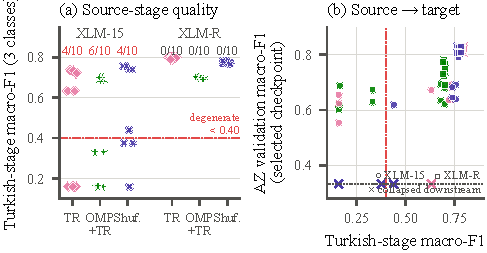
\includegraphics[width=\columnwidth]{figures/fig_turkish.pdf}
\caption{Turkish source stage (\file{results/aggregate.csv}). (a) Turkish validation \Fone{} (three classes) of every Turkish-bearing run; the count is degenerate stages per cell. (b) Downstream Azerbaijani validation \Fone{} against source-stage \Fone{} for the 60 Turkish-bearing runs; crosses are runs that collapsed downstream.}
\label{fig:turkish}
\end{figure}

\begin{table*}[!t]
\caption{Turkish-related contrasts on both bases (\file{results/stats.csv}). Escape gives escaped/declared seeds in baseline and comparison; $\Delta$ is conditional validation \Fone{} (comparison minus baseline, sign-adjusted when the stored orientation is reversed); ``shared'' is the number of seeds escaped in both arms; $\Delta$ test is the paired test difference on those seeds, recomputed from \file{results/runs/*.json}.}
\label{tab:turkish}
\centering
\footnotesize
\begin{tabular}{@{}lrlcrrrrrrrc@{}}
\toprule
Base & $n$ & Contrast & Escape & $\Delta$ cond. & Welch $p$ & Holm $p$ & Shared & Paired $p$ & $\Delta$ all-seed & $\Delta$ test & Surv. \\
\midrule
% AUTO-GENERATED by report/ieee/tables/make_tables.py -- do not edit by hand.
% source: results/stats.csv
% source: results/runs/*.json (paired test delta)
XLM-R & 500 & Direct $\to$ TR & 5/5, 5/5 & +0.0169 & 0.0034 & 0.1955 & 5 & 0.0021 & +0.0169 & +0.0127 &  \\
XLM-R & 500 & Direct $\to$ Shuf.\ TR & 5/5, 5/5 & +0.0073 & 0.1386 & 1 & 5 & 0.1091 & +0.0073 & +0.0031 &  \\
XLM-R & 500 & Shuf.\ TR $\to$ TR & 5/5, 5/5 & +0.0096 & 0.0483 & 1 & 5 & 0.0091 & +0.0096 & +0.0096 &  \\
XLM-R & 500 & Direct $\to$ OMP+TR & 5/5, 5/5 & -0.0720 & 0.0011 & 0.0631 & 5 & 0.0045 & -0.0720 & -0.0610 &  \\
XLM-R & 500 & OMP $\to$ OMP+TR & 5/5, 5/5 & +0.0062 & 0.5952 & 1 & 5 & 0.5386 & +0.0062 & +0.0138 &  \\
XLM-R & 500 & OMP+TR $\to$ TR & 5/5, 5/5 & +0.0889 & 5.0e-4 & 0.0310 & 5 & 0.0013 & +0.0889 & +0.0737 & \checkmark \\
\addlinespace[2pt]
XLM-R & 2,000 & Direct $\to$ TR & 5/5, 5/5 & +0.0030 & 0.3721 & 1 & 5 & 0.3755 & +0.0030 & +0.0078 &  \\
XLM-R & 2,000 & Direct $\to$ Shuf.\ TR & 5/5, 5/5 & -0.0008 & 0.8026 & 1 & 5 & 0.8254 & -0.0008 & +0.0001 &  \\
XLM-R & 2,000 & Shuf.\ TR $\to$ TR & 5/5, 5/5 & +0.0038 & 0.0377 & 1 & 5 & 0.0635 & +0.0038 & +0.0077 &  \\
XLM-R & 2,000 & Direct $\to$ OMP+TR & 5/5, 5/5 & -0.0569 & $<$1e-5 & $<$1e-5 & 5 & 2.9e-4 & -0.0569 & -0.0424 & \checkmark \\
XLM-R & 2,000 & OMP $\to$ OMP+TR & 5/5, 5/5 & +0.0090 & 0.1127 & 1 & 5 & 0.1756 & +0.0090 & +0.0142 &  \\
XLM-R & 2,000 & OMP+TR $\to$ TR & 5/5, 5/5 & +0.0599 & 1.0e-5 & 7.6e-4 & 5 & 2.0e-5 & +0.0599 & +0.0502 & \checkmark \\
\addlinespace[2pt]
\midrule
XLM-15 & 500 & Direct $\to$ TR & 3/5, 4/5 & -0.0165 & 0.4797 & 1 & 3 & 0.7542 & +0.0462 & +0.0070 &  \\
XLM-15 & 500 & Direct $\to$ Shuf.\ TR & 3/5, 3/5 & +0.0042 & 0.6784 & 1 & 2 & 0.5690 & +0.0025 & +0.0021 &  \\
XLM-15 & 500 & Shuf.\ TR $\to$ TR & 3/5, 4/5 & -0.0207 & 0.3939 & 1 & 2 & 0.9701 & +0.0437 & -0.0038 &  \\
XLM-15 & 500 & Direct $\to$ OMP+TR & 3/5, 5/5 & -0.0089 & 0.2924 & 1 & 3 & 0.4209 & +0.1100 & -0.0119 &  \\
XLM-15 & 500 & OMP $\to$ OMP+TR & 2/5, 5/5 & +0.0945 & 0.4728 & 1 & 2 & 0.4734 & +0.2108 & +0.0915 &  \\
XLM-15 & 500 & OMP+TR $\to$ TR & 5/5, 4/5 & -0.0076 & 0.7370 & 1 & 4 & 0.8427 & -0.0638 & -0.0039 &  \\
\addlinespace[2pt]
XLM-15 & 2,000 & Direct $\to$ TR & 2/5, 4/5 & -0.0044 & 0.6597 & 1 & 2 & 0.3488 & +0.1265 & -0.0096 &  \\
XLM-15 & 2,000 & Direct $\to$ Shuf.\ TR & 2/5, 2/5 & +0.0082 & 0.3605 & 1 & 0 & -- & -0.0049 & -- &  \\
XLM-15 & 2,000 & Shuf.\ TR $\to$ TR & 2/5, 4/5 & -0.0126 & 0.2440 & 1 & 1 & -- & +0.1315 & -0.0185 &  \\
XLM-15 & 2,000 & Direct $\to$ OMP+TR & 2/5, 5/5 & -0.0079 & 0.6001 & 1 & 2 & 0.8878 & +0.1913 & -0.0024 &  \\
XLM-15 & 2,000 & OMP $\to$ OMP+TR & 3/5, 5/5 & +0.0564 & 0.5342 & 1 & 3 & 0.4193 & +0.1689 & +0.0701 &  \\
XLM-15 & 2,000 & OMP+TR $\to$ TR & 5/5, 4/5 & +0.0035 & 0.8285 & 1 & 4 & 0.4582 & -0.0648 & -0.0079 &  \\
\addlinespace[2pt]
\bottomrule

\end{tabular}
\end{table*}

\subsection{Generalisation gap and validation–test agreement}
\label{sec:res:gap}
Across all 164 restored checkpoints the matched gap $\Delta=F_{\mathrm{test}}(t^\ast)-F_{\mathrm{val}}(t^\ast)$ has mean $-0.0126$, median $-0.0131$, standard deviation 0.0116, range $-0.0385$ to $+0.0095$, and is negative for 117 runs (Table~\ref{tab:gap}, Fig.~\ref{fig:valtest}). \xlmr{} runs have a larger gap (mean $-0.0202$, 69 of 70 negative) than \xlmxv{} runs ($-0.0069$), whose 34 collapsed runs contribute gaps near zero. A modest negative gap is the expected consequence of selecting the checkpoint on validation and supports treating the test split as confirmation rather than re-selection.

\begin{table}[!t]
\caption{Matched generalisation gap $F_{\mathrm{test}}-F_{\mathrm{val}}$ at the selected checkpoint (\file{results/aggregate.csv}).}
\label{tab:gap}
\centering
\scriptsize
\setlength{\tabcolsep}{2pt}
\begin{tabular}{@{}lrrrrrrr@{}}
\toprule
Subset & $N$ & Mean & Median & SD & Min & Max & $\Delta<0$ \\
\midrule
% AUTO-GENERATED by report/ieee/tables/make_tables.py -- do not edit by hand.
% source: results/aggregate.csv
All runs & 164 & -0.0126 & -0.0131 & 0.0116 & -0.0385 & +0.0095 & 117 \\
XLM-15 & 94 & -0.0069 & -0.0014 & 0.0101 & -0.0348 & +0.0095 & 48 \\
XLM-R & 70 & -0.0202 & -0.0202 & 0.0089 & -0.0385 & +0.0049 & 69 \\
Escaped runs & 130 & -0.0159 & -0.0163 & 0.0108 & -0.0385 & +0.0095 & 116 \\
Collapsed runs & 34 & +0.0000 & +0.0000 & 0.0018 & -0.0076 & +0.0069 & 1 \\
\bottomrule

\end{tabular}
\end{table}

\begin{figure*}[!t]
\centering
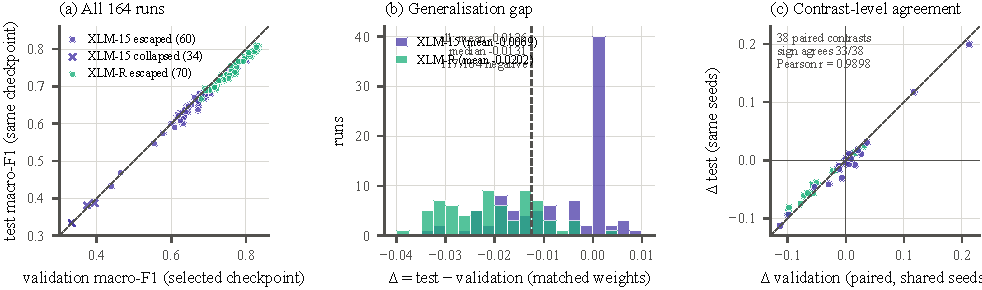
\includegraphics[width=\textwidth]{figures/fig_valtest.pdf}
\caption{Validation against test. (a) Selected-checkpoint validation \Fone{} versus test \Fone{} for all 164 runs (\file{results/aggregate.csv}). (b) Distribution of the matched gap. (c) Contrast-level agreement: paired validation difference versus paired test difference for the 38 contrasts with at least one shared escaped seed (T2 of \file{test\_tables\_received.md}).}
\label{fig:valtest}
\end{figure*}

\subsection{Fixed-step data-size sensitivity (\xlmxv)}
\label{sec:res:size}
Table~\ref{tab:size} extends the four non-Turkish \xlmxv{} conditions to $n=10{,}000$ and $n=20{,}914$ with three seeds. Escape is non-monotonic in $n$: \Direct{} escapes 3/5, 2/5, 2/3 and 3/3; \OMP{} 2/5, 3/5, 3/3 and 1/3; \Mean{} 2/5, 3/5, 1/3 and 3/3; \Random{} 3/5, 4/5, 1/3 and 1/3. At $n=20{,}914$ the single escaped \OMP{} seed reaches a conditional 0.7900 while the cell's all-seed value is 0.4856, a direct example of selection-induced ranking distortion. Because every cell receives 2{,}000 steps, exposure falls from about 125 passes to 3 across the sweep; the table is a fixed-budget robustness probe, and cells with one escaped seed have only descriptive conditional values. The only measurable higher-data contrast, \Direct$\to$\OMP{} at $n=10{,}000$ ($+0.0230$, Welch $p=0.112$), does not survive correction. H2 therefore receives no support in the form it was stated: the transplant does not help the encoder that lacks Azerbaijani pretraining, and on that encoder it is not distinguishable from its placebos.

\begin{table}[!t]
\caption{\xlmxv{} fixed-step size sensitivity (\file{results/summary.csv}, T1 of \file{test\_tables\_received.md}); five seeds at $n\le2{,}000$, three above.}
\label{tab:size}
\centering
\scriptsize
\begin{tabular}{@{}rlcrrrr@{}}
\toprule
 & & & \multicolumn{2}{c}{Validation \Fone} & \multicolumn{2}{c}{Test \Fone} \\
\cmidrule(lr){4-5}\cmidrule(lr){6-7}
$n$ & Condition & Escape & cond. & all-seed & cond. & all-seed \\
\midrule
% AUTO-GENERATED by report/ieee/tables/make_tables.py -- do not edit by hand.
% source: results/summary.csv
% source: test_tables_received.md (T1)
500 & Direct & 3/5 & 0.6306 & 0.5117 & 0.6229 & 0.5071 \\
500 & OMP & 2/5 & 0.5272 & 0.4109 & 0.5248 & 0.4100 \\
500 & Mean & 2/5 & 0.6359 & 0.4544 & 0.6302 & 0.4521 \\
500 & Random & 3/5 & 0.6192 & 0.5049 & 0.6025 & 0.4949 \\
\addlinespace[2pt]
2,000 & Direct & 2/5 & 0.6791 & 0.4799 & 0.6735 & 0.4790 \\
2,000 & OMP & 3/5 & 0.6148 & 0.5023 & 0.6076 & 0.4980 \\
2,000 & Mean & 3/5 & 0.6955 & 0.5507 & 0.6833 & 0.5434 \\
2,000 & Random & 4/5 & 0.6699 & 0.6026 & 0.6529 & 0.5890 \\
\addlinespace[2pt]
10,000 & Direct & 2/3 & 0.7427 & 0.6063 & 0.7253 & 0.5947 \\
10,000 & OMP & 3/3 & 0.7657 & 0.7657 & 0.7438 & 0.7438 \\
10,000 & Mean & 1/3 & 0.7653 & 0.4774 & 0.7539 & 0.4736 \\
10,000 & Random & 1/3 & 0.6319 & 0.4533 & 0.6129 & 0.4444 \\
\addlinespace[2pt]
20,914 & Direct & 3/3 & 0.7374 & 0.7374 & 0.7217 & 0.7217 \\
20,914 & OMP & 1/3 & 0.7900 & 0.4856 & 0.7735 & 0.4801 \\
20,914 & Mean & 3/3 & 0.7263 & 0.7263 & 0.7062 & 0.7062 \\
20,914 & Random & 1/3 & 0.7671 & 0.4780 & 0.7417 & 0.4695 \\
\bottomrule

\end{tabular}
\end{table}

\subsection{Error taxonomy on test predictions}
\label{sec:res:errors}
An automatic keyword taxonomy assigns each misclassified test example at $n=2{,}000$, pooled over both bases and all five seeds (41{,}860 predictions per condition), to one of four categories (\file{src/analysis/errors.py}), in order of precedence: false friend (the text contains a word from a Turkish–Azerbaijani false-friend list, ile{resources/false\_friends.csv}), technical vocabulary (a short list of language-reform vocabulary pairs), morphological (the example's tokens per word under the primary tokenizer exceed 4, a proxy for long suffix chains), or other (Table~\ref{tab:errors}, Fig.~\ref{fig:errors}). Error rates track the aggregate \Fone{}: 28.0\% for \TR, 29.0\% for \OMPTR, 31.5–31.6\% for \Direct, \Mean{} and \ShufTR, 33.1\% for \Random{} and 34.1\% for \OMP. The category shares are nearly identical across conditions (morphological 5.8–6.5\%, technical 1.4–1.6\%, false friend 0.2–0.3\%, other 91.8–92.3\%): the interventions change \emph{how many} errors are made, not the keyword profile of the errors. Because the taxonomy is lexical and 92\% of errors fall outside its lists, we treat it as a null result about keyword-defined error types rather than as a characterisation of the errors; a 210-row manual sample (\file{errors\_manual\_sample.csv}) was exported but not annotated within the project window.

\begin{table}[!t]
\caption{Automatic error taxonomy on test predictions at $n=2{,}000$, both bases and all seeds pooled (\file{results/errors.json}). Shares are percentages of errors.}
\label{tab:errors}
\centering
\scriptsize
\setlength{\tabcolsep}{2pt}
\begin{tabular}{@{}lrrrrrrr@{}}
\toprule
 & & & Error & \multicolumn{4}{c}{Share of errors (\%)} \\
\cmidrule(lr){5-8}
Condition & Evaluated & Errors & rate (\%) & Morph. & Techn. & False fr. & Other \\
\midrule
% AUTO-GENERATED by report/ieee/tables/make_tables.py -- do not edit by hand.
% source: results/errors.json
Direct & 41,860 & 13,176 & 31.48 & 6.5 & 1.4 & 0.2 & 91.8 \\
OMP & 41,860 & 14,286 & 34.13 & 6.0 & 1.6 & 0.3 & 92.1 \\
Mean & 41,860 & 13,221 & 31.58 & 5.9 & 1.5 & 0.3 & 92.3 \\
Random & 41,860 & 13,852 & 33.09 & 6.0 & 1.6 & 0.3 & 92.0 \\
TR & 41,860 & 11,736 & 28.04 & 6.2 & 1.5 & 0.3 & 92.0 \\
OMP+TR & 41,860 & 12,137 & 28.99 & 5.8 & 1.6 & 0.3 & 92.2 \\
Shuf. TR & 41,860 & 13,196 & 31.52 & 6.4 & 1.4 & 0.3 & 91.9 \\
\bottomrule

\end{tabular}
\end{table}

\begin{figure}[!t]
\centering
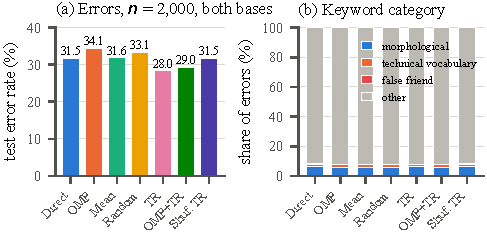
\includegraphics[width=\columnwidth]{figures/fig_errors.pdf}
\caption{Error taxonomy at $n=2{,}000$ (\file{results/errors.json}). (a) Test error rate per condition, both bases and all seeds pooled. (b) Keyword category shares; ``other'' dominates in every condition.}
\label{fig:errors}
\end{figure}

\subsection{Compute cost per condition}
\label{sec:res:cost}
Per-run wall-clock (Fig.~\ref{fig:runtime}, Table~\ref{tab:compute}) is governed by the encoder and the vocabulary: \xlmxv{} runs take 2.9–3.6 minutes and \xlmr{} runs 2.5–6.8 minutes, with the transplanted-vocabulary conditions slightly faster than the original-vocabulary ones because the tied output projection is smaller. The four data sizes differ little in wall-clock because the step budget is fixed. The whole grid consumed 8.36 process-hours on one GPU.
